\documentclass[11pt]{article}
\usepackage[margin=1in]{geometry}
\usepackage{amsmath,amssymb,booktabs,graphicx,caption,hyperref,siunitx}
\newcommand{\rel}{\mathrm{relerr}}
\title{Local-KLE (MSM) pCN samplers, round 2: speed versus posterior fidelity}
\date{4 November 2026}
\begin{document}
\maketitle

\section{Summary of findings}
This report covers the 15 runs of Table~1: the second-round experiments and the re-run first-pass experiments (all 64 chains, $10^5$ iterations, $M=10^4$ adaptation iterations, state saved every 50 iterations except experiments 4 and 5, saved every 100). The setup, rank test and prior test are in the first report (\texttt{msm\_local\_kle\_report.pdf}) and are not repeated.
\begin{itemize}
\item \textbf{Only experiment 3b reproduces the global posterior.} Its mean posterior standard deviation of $\log\kappa$ is $0.576$ against $0.570$ for global pCN, and its error of the posterior-mean field is $0.409$ against $0.416$. Every other local-KLE sampler is narrower: by $10$--$17\%$ (ratios $0.83$--$0.90$) for all except the mixtures 4 and 4.8, which collapse (ratios $0.38$ and $0.44$). Their mean fields are also further from the truth ($0.42$--$0.50$, and $0.56$ for the mixtures).
\item \textbf{Speed and fidelity trade off, as you expected.} 3b reaches MPSRF $<1.2$ after $51$k iterations against $56$k for global pCN (about $9\%$ faster, a single replicate, so within plausible noise). The under-dispersed samplers (excluding the mixtures) reach it after $28$--$45$k. The fastest honest alternative, alternating with no offset (6d), needs $29$k, about $48\%$ fewer iterations than global pCN, but it samples a distribution about $14\%$ too narrow.
\item \textbf{Experiment 4 is not rescued by a larger local dimension.} With 8 local modes per block the primal acceptance rises from $0.16\%$ to $25\%$, but the posterior spread is still only $0.44$ of the global one and the median relative error is $0.030$ against the $0.0204$ plateau of every other run. Raising the local dimension therefore does not remove the failure; the projection $\Pi_g$ at every switch is the likely cause (Section~\ref{sec:exp4}).
\item \textbf{The innovation form of the mixture (4b) and all alternating schemes (6a--6d) are well behaved}: acceptance $\approx25\%$ in both grids, plateau relative error $0.0203$--$0.0204$, MPSRF below $1.1$ in the 58 range coordinates. They share the under-dispersion (ratio $0.86$--$0.89$) of the raw primal sampler and are not prior preserving.
\item \textbf{The number of inner iterations $L$ and the frozen-offset move matter little.} $L=1,10,100$ reach MPSRF $<1.2$ at $37$k, $36$k, $42$k; dropping the offset (6d) is fastest ($29$k) but also gives a slightly narrower posterior ($0.86$) than the offset versions ($0.88$--$0.89$).
\end{itemize}

\section{Experiments and how MPSRF is computed}
\begin{center}\small
\begin{tabular}{@{}lp{0.78\textwidth}@{}}\toprule
1 & global pCN on $\theta\in\mathbb R^{64}$\\
2, 2.6, 2.8 & primal raw, $\theta=Bc$; $4$, $6$, $8$ local modes per $4\times4$ block ($p=64,96,128$)\\
3a, 3b & whitened pseudo-inverse; whitened plus null-space term $V_0\zeta$ (exact prior)\\
4, 4.8 & mixture primal/dual through the global state with projection $\Pi_g$ (4 and 8 local modes)\\
4b & mixture, innovation form $\theta'=\sqrt{1-s^2}\,\theta+s\,B_g\xi$\\
5, 5b & $5\cdot10^4$ primal iterations then $5\cdot10^4$ dual; switch by $\Pi_{\rm dual}$ (5) or the exact lift $L_d$ (5b)\\
6a--6c & alternating primal/dual blocks of $L=1,10,100$ iterations, frozen-offset move $\theta'=\theta+B_g(c'-c_0)$, $c_0=L_g\theta$\\
6d & as 6a but without the offset ($\theta'=B_gc'$ in the primal block)\\ \bottomrule
\end{tabular}
\end{center}
\textbf{MPSRF and PSRF (group convention, \texttt{brho/mpsrf.py}).} The window starts at iteration $1000$ (of the phase, for phase 2 of experiment 5), so the adaptation period is \emph{not} discarded, and it grows to the end of the run: at each curve point it holds the saved samples from the start to the current iteration, every 2nd sample, with a curve point every 15 saved samples. $W$ is the average within-chain covariance (divisor $n-1$), $B/n$ the covariance of the chain means (divisor $m-1$), $\mathrm{MPSRF}=\sqrt{(n-1)/n+(m+1)/m\,\lambda_{\max}(W^{-1}B/n)}$, and PSRF$_i=\sqrt{V_{ii}/W_{ii}}$ with the maximum over components reported. Not split-chain, no extra burn-in. ``Iterations to $1.2$'' is the first curve point (ignoring the first 10) below $1.2$, linearly interpolated. For comparability all runs are measured on the same 58 coordinates $V_+^\top\theta$ of the rank-58 range (``common 58''); for experiment 2 and 3a, whose $\theta$ lies in that range, these are the natural coordinates, and for experiment 2.6, 2.8 and 4.8 the 64-dimensional $\theta$ is used (the common-58 entry coincides with it). For phase 2 of experiments 5 and 5b the count is in iterations after the switch.

\section{Results}
\begin{table}[h]\centering\small
\resizebox{\textwidth}{!}{\begin{tabular}{@{}lccccccccc@{}}\toprule
run & acc.\ (primal/dual) & median $\rel$ & iter.\ to 1.2 (k) & MPSRF end & max PSRF end & mean sd $\log\kappa$ & ratio to 1 & rms err.\ mean\\ \midrule
1 global & 0.25 & 0.0205 & 56.1 & 1.115 & 1.052 & 0.570 & 1.00 & 0.416 \\
2 primal raw d4 & 0.25 & 0.0204 & 37.2 & 1.072 & 1.033 & 0.474 & 0.83 & 0.496 \\
2.6 primal raw d6 & 0.26 & 0.0204 & 45.2 & 1.081 & 1.044 & 0.491 & 0.86 & 0.479 \\
2.8 primal raw d8 & 0.26 & 0.0204 & 37.7 & 1.072 & 1.039 & 0.500 & 0.88 & 0.477 \\
3a pinv & 0.25 & 0.0204 & 45.2 & 1.083 & 1.042 & 0.512 & 0.90 & 0.457 \\
3b aug & 0.26 & 0.0205 & 51.2 & 1.110 & 1.048 & 0.576 & 1.01 & 0.409 \\
4 mixture d4 & 0.00/0.25 & 0.0332 & 22.7 & 1.397 & 1.084 & 0.217 & 0.38 & 0.556 \\
4.8 mixture d8 & 0.25/0.25 & 0.0300 & 15.9 & 1.280 & 1.037 & 0.250 & 0.44 & 0.562 \\
4b mixture innov. & 0.25/0.24 & 0.0203 & 37.3 & 1.064 & 1.031 & 0.500 & 0.88 & 0.431 \\
5 sequence & 0.25/0.27 & 0.0205 & 33.0 & 1.131 & 1.067 & 0.491 & 0.86 & 0.446 \\
5b sequence exact & 0.25/0.26 & 0.0205 & 27.9 & 1.125 & 1.053 & 0.491 & 0.86 & 0.451 \\
6a alt L=1 & 0.25/0.25 & 0.0204 & 37.1 & 1.085 & 1.035 & 0.504 & 0.88 & 0.425 \\
6b alt L=10 & 0.25/0.26 & 0.0204 & 35.8 & 1.077 & 1.035 & 0.508 & 0.89 & 0.427 \\
6c alt L=100 & 0.26/0.27 & 0.0204 & 41.6 & 1.072 & 1.031 & 0.504 & 0.88 & 0.421 \\
6d alt L=1 no offset & 0.25/0.23 & 0.0204 & 29.2 & 1.060 & 1.036 & 0.490 & 0.86 & 0.440 \\
\bottomrule\end{tabular}}
\caption{All runs. Fields use 10{,}000 pooled samples after adaptation (5{,}000 per phase for experiments 5, 5b, pooled here). ``ratio to 1'' is the mean posterior sd of $\log\kappa$ divided by that of experiment 1; ``rms err.\ mean'' is the rms difference between the posterior-mean $\log\kappa$ field and the truth. For experiments 4 and 4.8 the ``iter.\ to 1.2'' entry is a false crossing (Section~\ref{sec:exp4}).}
\end{table}

\begin{figure}[h]\centering
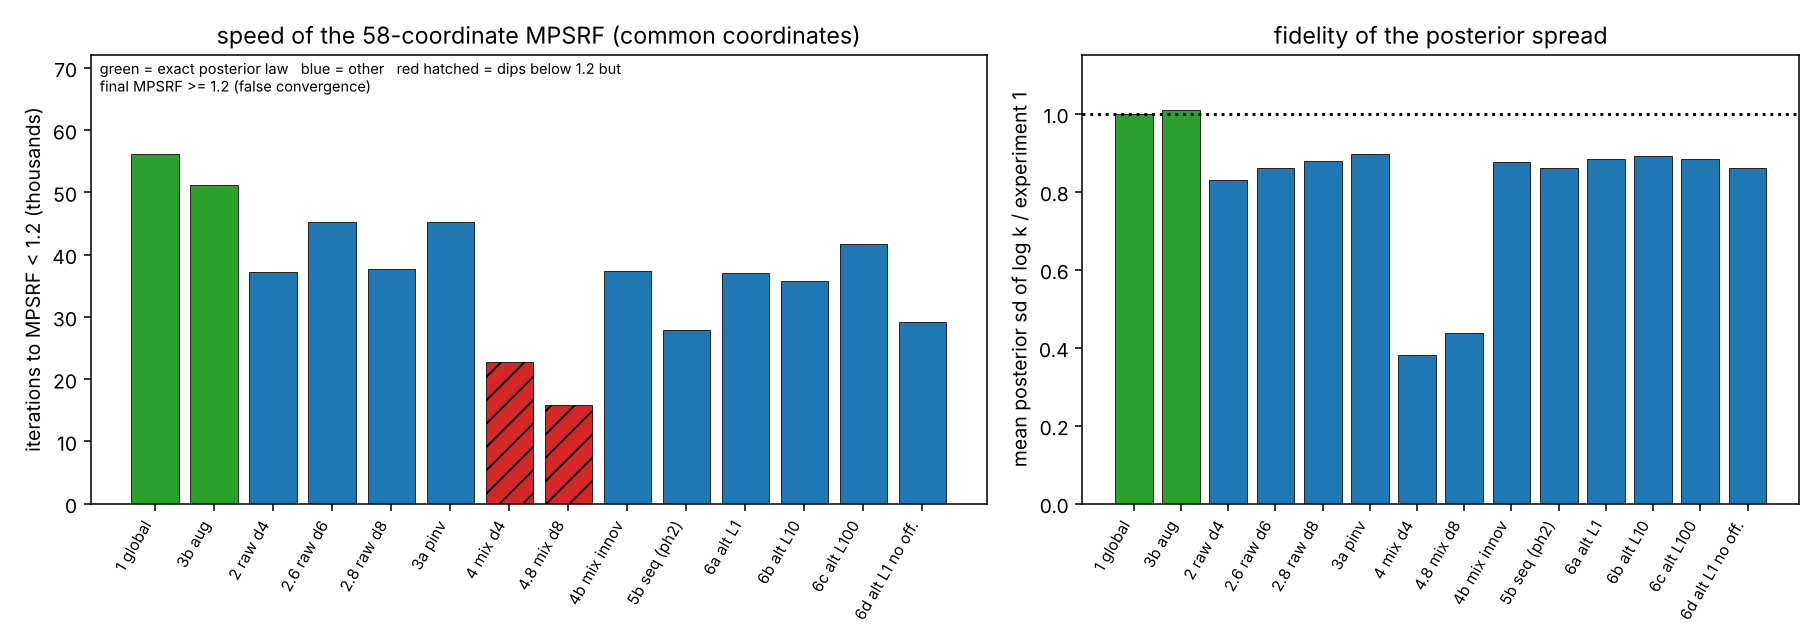
\includegraphics[width=\textwidth]{fig2/fig_conv_bar.png}
\caption{Left: iterations to MPSRF $<1.2$ (58 common coordinates). Right: mean posterior sd of $\log\kappa$ relative to global pCN. The two samplers that preserve the posterior (green) are the slowest; everything faster is also narrower.}
\end{figure}

\subsection{Speed comes with variance loss}
The relationship in Figure~1 is the central result. The raw primal sampler (2) and the whitened pseudo-inverse sampler (3a) are faster than global pCN, and both have the narrower posterior of the model they actually sample, $N(0,\Sigma_{ms})$ or $N(0,V_+V_+^\top)$. In the standard-deviation maps (Figure~2) experiment 2 shows an imprint of the $4\times4$ blocks that is absent in the global and 3b maps, and the maps of the alternating and innovation samplers (6a, 6d, 4b) are close to each other and slightly flatter than the global one. Adding the null-space term (3b) restores the target exactly and takes the speed advantage with it, apart from a modest remainder.

Eight local modes per block (2.8) raises the ratio from $0.83$ to $0.88$ and keeps the speed of experiment 2 ($37.7$k against $37.2$k); six modes (2.6) is in between in spread but slower ($45$k). With one replicate per setting I would not read the ordering $37<45<38$k among 2, 2.6 and 2.8 as meaningful.

\begin{figure}[h]\centering
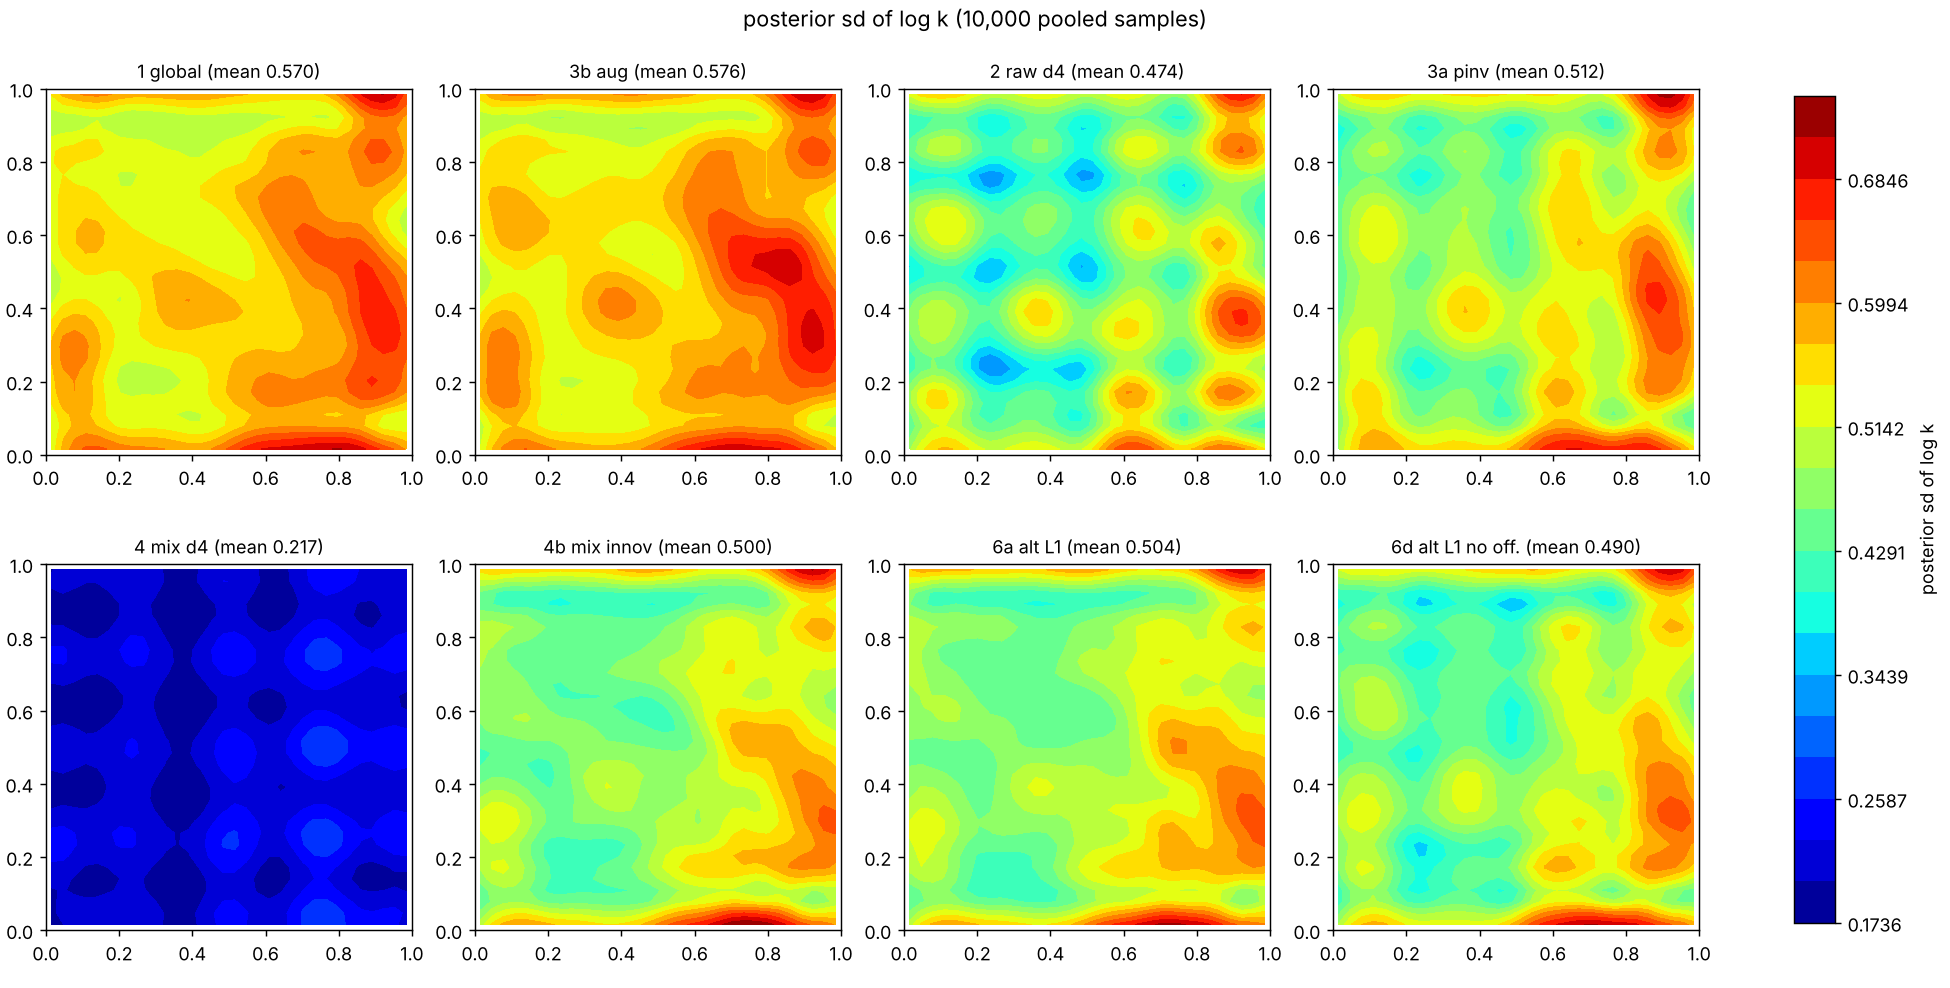
\includegraphics[width=\textwidth]{fig2/fig_logk_sd_grid.png}
\caption{Posterior sd of $\log\kappa$, shared colour scale (jet, contourf), eight representative runs.}
\end{figure}

\subsection{Experiment 4: why larger local dimension does not fix it}\label{sec:exp4}
In experiment 4 the primal proposals are almost never accepted ($0.16\%$ against $25\%$ for dual) and the median relative error is $0.033$, the chains sitting above the posterior plateau. Its MPSRF curve (Figure~3, left) dips to about $1.18$ near $25$k iterations and then rises to $1.40$, so the ``$22.7$k'' in Table~1 is a transient crossing, not convergence. Raising the local dimension to 8 (4.8) makes both grids accept at $25\%$, but the sd ratio is only $0.44$, the median relative error is $0.030$ and the final MPSRF is $1.28$. The acceptance problem was therefore a symptom; a likely explanation, which these runs support but do not prove, is that the projection $\Pi_g$ at every switch removes information from $\theta$ that the other grid cannot restore, so the state contracts. The innovation form (4b), which never projects the current state, does not show the failure: relative error $0.0203$, ratio $0.88$.

\begin{figure}[h]\centering
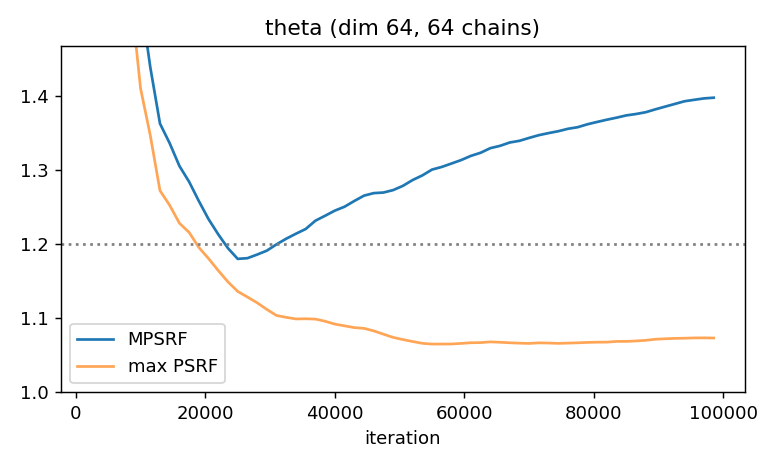
\includegraphics[width=0.49\textwidth]{fig2/mpsrf_exp4.png}\hfill
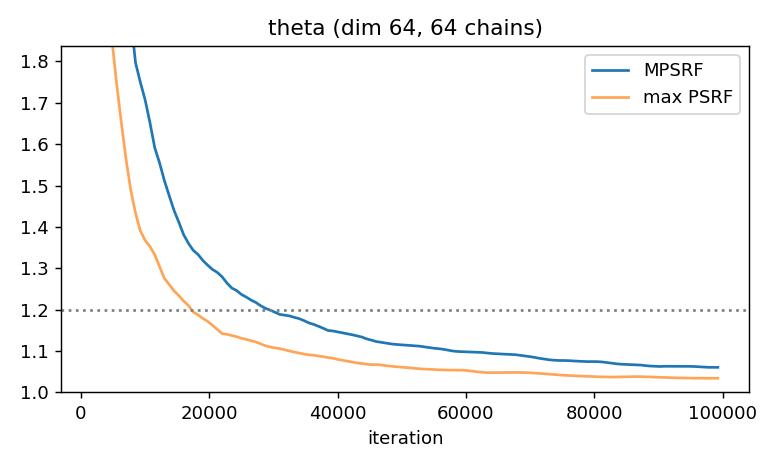
\includegraphics[width=0.49\textwidth]{fig2/mpsrf_exp6d.png}
\caption{MPSRF and max PSRF of $\theta$ (64 dimensions). Left: experiment 4 (dips below $1.2$, then rises). Right: experiment 6d (monotone decrease, crosses $1.2$ at about $29$k).}
\end{figure}

\subsection{Alternating samplers and the primal$\to$dual sequence}
The alternating schemes are not prior preserving: the earlier stationary-covariance analysis gave a pointwise \emph{prior} variance ratio of about $0.77$ for them. The measured \emph{posterior} sd ratios here ($0.86$--$0.89$, variance ratios $0.74$--$0.79$) are of the same size, although they are different quantities. Block length $L$ and the offset change the speed a little ($29$--$42$k) and the spread hardly at all. For the sequence, phase 1 reaches $1.2$ at about $37$k iterations and phase 2, measured in the window beginning $1000$ iterations after the switch, at $33$k (5) and $28$k (5b, exact lift) iterations after the switch. The difference between 5 and 5b is of a size I would expect from run-to-run noise.

\subsection{Mean-field accuracy}
The error of the posterior-mean $\log\kappa$ field relative to the truth is lowest for 3b ($0.409$) and global pCN ($0.416$), $0.42$--$0.46$ for the alternating, innovation, 3a and sequence samplers, $0.48$--$0.50$ for the raw primal runs, and $0.56$ for the mixtures. Figure~4 shows the corresponding mean maps. The differences among the middle group are small compared with the noise expected from a single data set and seed.

\begin{figure}[h]\centering
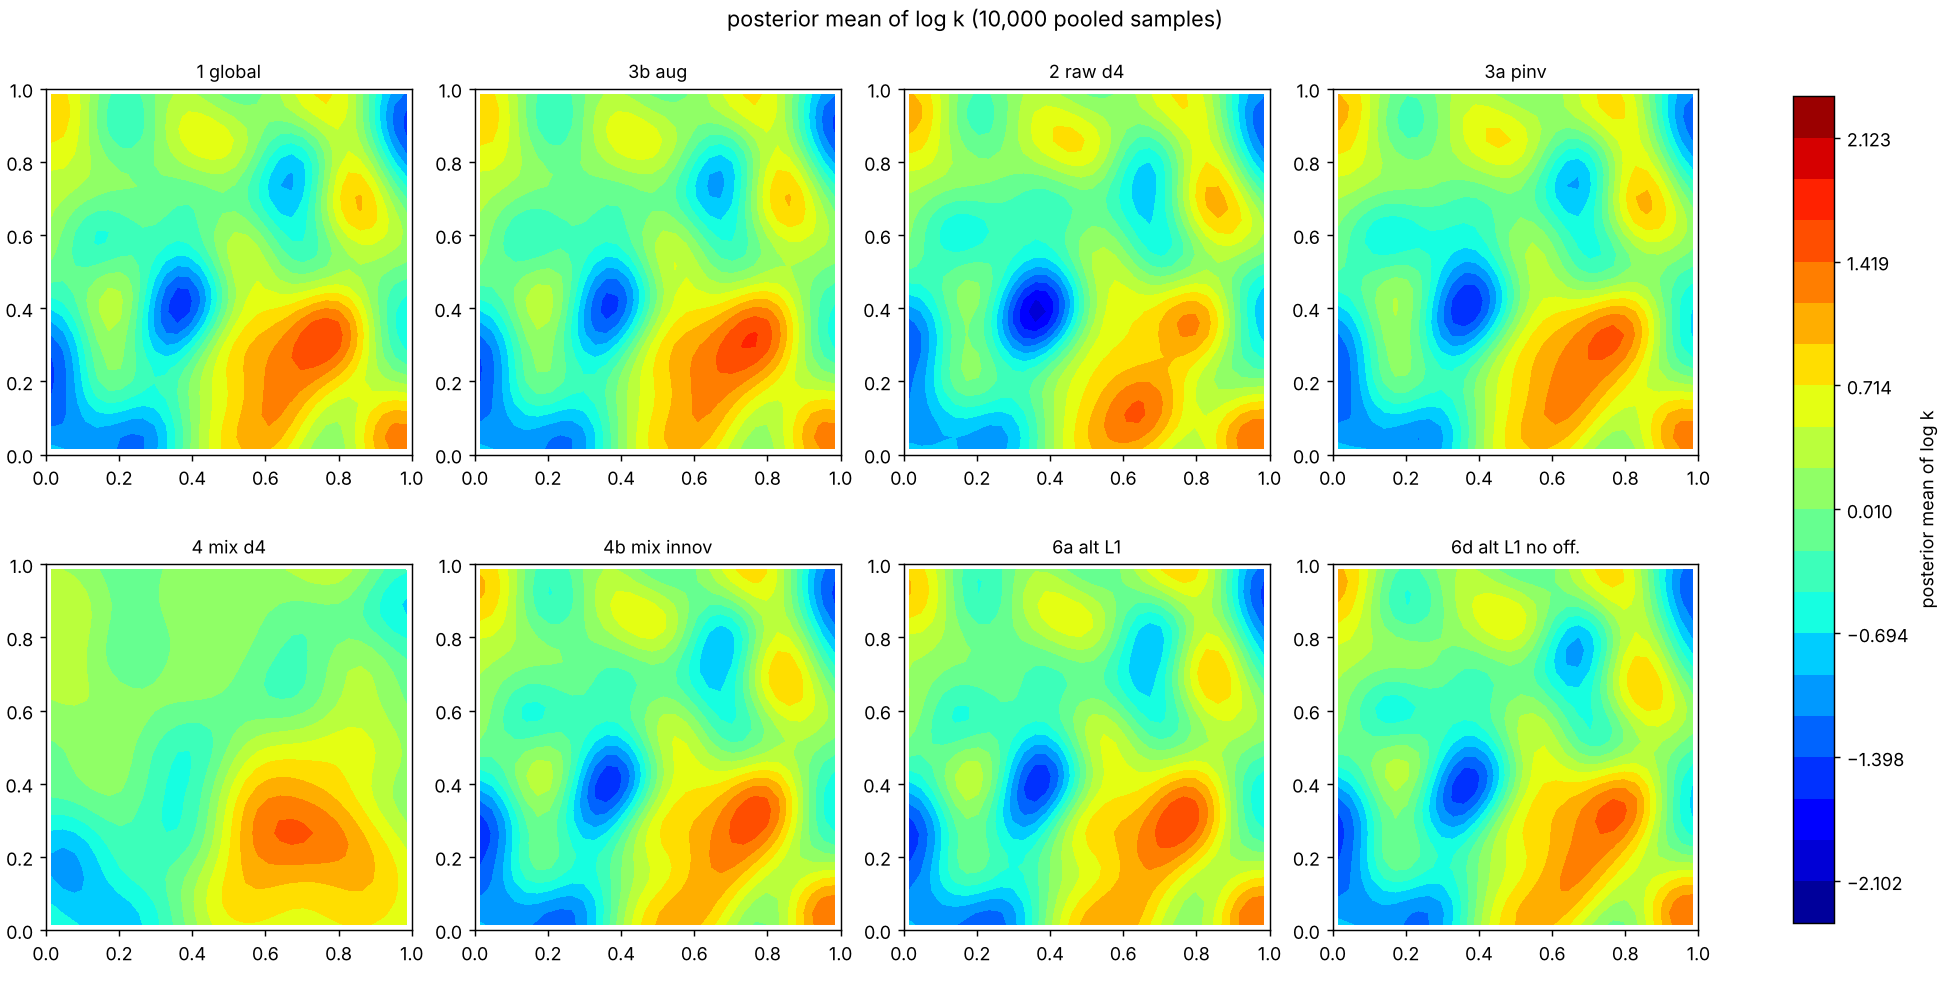
\includegraphics[width=\textwidth]{fig2/fig_logk_mean_grid.png}
\caption{Posterior mean of $\log\kappa$ (shared scale) for the same eight runs.}
\end{figure}

\section{Caveats}
\begin{itemize}
\item \textbf{One replicate, one data set.} Every run uses 64 chains from a single seed set and one noisy data set. Differences of $10$--$15\%$ in iterations to $1.2$ (for example 5 against 5b, or 2 against 2.8) are not distinguishable from noise here; the speed differences of $20$--$48\%$ for the non-mixture samplers relative to global pCN and the sd ratios of $0.83$--$0.90$ against $1.01$ for 3b are larger, but a second seed set would confirm them.
\item \textbf{The sd comparison uses correlated samples.} It is a pooled posterior sd of $10^4$ saved states; the ratio of 3b to 1 ($1.01$) is consistent with a Monte Carlo error of order a percent, but one pair of runs cannot establish it.
\item \textbf{MPSRF in the 114 dual coordinates.} The post-processing also reports MPSRF of the dual local coefficients $\Pi_d\theta$ or $L_d\theta$ (114 coordinates, rank 64, files \texttt{post\_summary.json} entries \texttt{c\_dual\_proj}), with values up to $1.95$. Their within-chain covariance is singular, so these numbers are numerically unreliable and I do not use them. The 64-coordinate primal projections (rank 58) share the issue in milder form. The \emph{state} coefficients of experiments 2, 2.6, 2.8, 3a, 3b and phase~1 of 5 are full rank and are reported in \texttt{post\_summary.json}.
\item \textbf{The fidelity measure is the sd of $\log\kappa$ only.} I did not compare higher moments or the posterior of the data fit.
\end{itemize}

\section{Interpretation and next steps}
For the rank-58 primal basis, local-KLE pCN is faster than global pCN only to the extent that it fails to sample some of the long-range variance; with the exact prior restored (3b) the gain is small. If the aim is a fast, exact sampler, the results suggest looking for a version of the alternating scheme with a correction step that restores the prior covariance; this has not been tested. If an approximate posterior with bounded variance loss is acceptable, the alternating no-offset sampler (6d) gives the fastest mixing here. For experiment 4 as defined (projection through the global state), the results argue for abandoning it in favour of 4b.

\paragraph{Reproduction.} The scripts \texttt{make\_msm\_round2\_table.py} and \texttt{make\_msm\_round2\_figures.py} (in \texttt{experiments/}) read only the committed \texttt{summary.json}, \texttt{post\_summary.json} and \texttt{fields.npz} files. Run them with the environment variable \texttt{BRHO\_ROOT} set to \texttt{runs/msm\_local\_kle\_2026-11}.
\end{document}
